%%
%% Interaction 2024 Technical Report Submission
%% V1.6 (2023/12/22)
%% 

\documentclass[submit,techrep,english]{ipsj}


\usepackage{graphicx}
\usepackage{latexsym}
\usepackage{url}


\def\Underline{\setbox0\hbox\bgroup\let\\\endUnderline}
\def\endUnderline{\vphantom{y}\egroup\smash{\underline{\box0}}\\}
\def\|{\verb|}

\setcounter{volume}{64}%vol53=2012
\setcounter{number}{10}
\setcounter{page}{1}

% インタラクション特有の設定。印刷工程で柱・ノンブルの埋め込みを行う。
\makeatletter
\pagestyle{empty}
\def\@oddhead{}%
\def\@evenhead{}%
\def\ps@IPSJTITLEheadings{}
\makeatother


\begin{document}


\title{MyStoryKnight: A Character-drawing Driven Storytelling System Using LLM Hallucinations}

\affiliate{LU}{Lund University}
\affiliate{TUD}{Technical University of Denmark}
\affiliate{HRI}{Honda Research Institute Japan}
\affiliate{UTokyo}{The University of Tokyo}
\paffiliate{PUTokyo}{The University of Tokyo}

\author{Sechayk Yotam}{UTokyo}[sechayk-yotam@g.ecc.u-tokyo.ac.jp]
\author{Penarska Gabriela A.}{TUD,PUTokyo}[gabriela-penarska@g.ecc.u-tokyo.ac.jp]
\author{Randsalu Isa A.}{LU,PUTokyo}[randsalu-isa071@g.ecc.u-tokyo.ac.jp]
\author{Arzate Cruz Christian}{HRI}[]
\author{Igarashi Takeo}{UTokyo}[]


\begin{abstract}
    Storytelling is a valuable tradition that plays a crucial role in child development, fostering creativity and a sense of agency. However, many children often consume stories passively, missing out on the opportunity to participate in the creative process. To address this, we propose a storytelling system that creates adventure-type stories with multiple branches that users can explore. We generate these interactive stories using a character drawing as input, with visual features extraction using GPT-4. By leveraging LLM hallucinations, we generate interactive stories using user feedback as a prompt. Finally, we refine the quality of the generated story through a complexity analysis algorithm. We believe that the use of a drawing as input further improves the engagement in the story and characters.
\end{abstract}

\maketitle

%1
\section{Introduction}
\label{sec:introduction}
Creativity is increasingly recognized as a crucial aspect of the modern working environment. In the context of child development, creativity plays a pivotal role in fostering learning and growth \cite{1:ElgarfP22}, which extends to adulthood. As a result, there has been a growing interest in leveraging creative artificial intelligence (AI) and exploring the use of AI agents to stimulate children's creativity. Previous research has demonstrated the positive effects of incorporating AI agents with creative abilities in enhancing children's creative thinking. Additionally, the use of storytelling robots and virtual characters as interactive tools has gained traction in recent years \cite{7:SunLLL17}. In this paper, we propose \textit{MyStoryKnight}, an interactive AI tool for generating stories.

Our proposed system is intended to promote children's creativity through storytelling, a popular activity for entertaining and bonding \cite{7:SunLLL17}. Both storymaking and storytelling contribute to the development of verbal and social skills \cite{9:RyokaiC99,5:CurrinDPCFGH23}, such as broadening the vocanulary and improving  narrative comprehension. Besides, creating fictional worlds and characters helps children improve their language skills, both in comprehension and usage \cite{13:abs-2011-04242}. In \textit{MyStoryKnight}, users, together with an AI, co-create stories with multiple explorable branches.

Despite all the benefits of practicing storytelling, many children do not have the opportunity to engage in interactive storytelling. \textit{MyStoryKnight} addresses this problem by generating an adventure-type story through LLM hallucinations. Figure \ref{fig:system-overview}  shows an overview of our system. Our system uses drawings of characters as input, and generates an unfolding story that the user can navigate through based on their choices. Using a complexity analysis algorithm, we guide the LLM hallucinations to generate a coherent and consistent story. Resulting in a story that is both engaging and easy to follow.

\begin{figure*}[t]
    \centering
    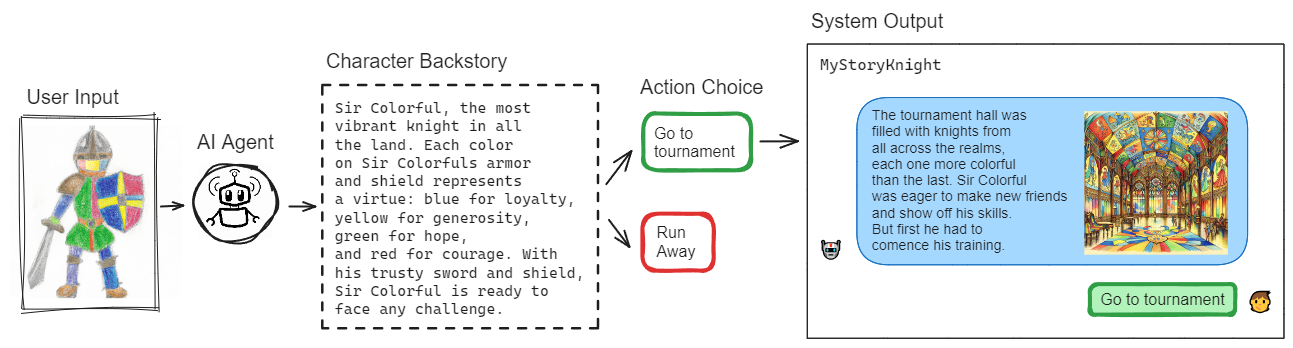
\includegraphics[width=0.95\textwidth]{figures/system-overview.png}
    \caption{MyStoryKnight system overview. Drawing is anaylzed with GPT-4. Backstory and action choices are presented to the user. Story unfolds based on user choice.}
    \label{fig:system-overview}
\end{figure*}

Our contributions are:
\begin{itemize}
    \item Storytelling system that uses the character drawing as a basis for the story.
    \item LLM hallucinations to generate an adventure-type story with user navigation.
    \item Complexity analysis of story generation for coherency and consistency.
\end{itemize}


%2
\section{Related Work}
\label{sec:related-work}

\subsection{Interactive Storytelling}
Interactive storytelling is a form of storytelling in which the audience is an active participant \cite{14:WangRCRMB22}. Interactive storytelling has been shown to be an effective way of building and strengthening relationships \cite{15:SchlauchSG22}, playing an important role in parent-child bonding \cite{12:ZhangXWYRWYWL22}. Interactive stories stimulate thinking and imagination \cite{11:LimaGV20}, and help children make sense of their world through shared experiences \cite{9:RyokaiC99}.

Prior work has explored physical interactivity through the use of tangible objects to create stories \cite{9:RyokaiC99}, and physical gestures to control characters \cite{2:LiuLWCS12} or create stories \cite{3:ZhaoB23}. Other studies have explored the use of sketches to influence character behavior and plot development \cite{11:LimaGV20}.

However, these studies have not explored the use of tangible character drawings made by users as the driving force behind the story.

\subsection{AI Storytelling}
AI usage has been experiencing a surge in popularity in recent years, with many applications in the creative arts. Generative AI especially has the potential to contribute to creative processes \cite{6:TholanderJ23}. One such creative process could be storytelling.

Prior work has explored how generative AI can be used to create stories \cite{13:abs-2011-04242}, and even collaborate in story generation with other humans \cite{8:ShakeriND21}. Other studies explored how generative AI can be used to expand existing story worlds \cite{10:ChopraVSS21}, or generate comprehensive multi-modal storytelling experiences \cite{4:HanC23}.

However, while consistency and coherency are essential in storytelling, they are often overlooked in AI-generated stories.

\subsection{Storytelling with Children}
Children oriented storytelling has been widely explored in the past. Prior work has examimned the use of robots as storytelling companions \cite{7:SunLLL17}, and the use of virtual characters to promote collaboreation \cite{2:LiuLWCS12}. Other studies have explored the use of AI agents to stimulate children's creativity \cite{1:ElgarfP22}, or show how AI can support parent-child bonding \cite{12:ZhangXWYRWYWL22}. Moreover, storytelling with AI-agents can encourage physical interaction and play \cite{3:ZhaoB23}.

However, utilizing LLM hallucinations to generate stories has not been explored in the context of user-agency for storytelling with children.

%3
\section{System Overview}
\label{sec:system-overview}
We designed \textbf{MyStoryKnight}, an interactive storytelling that uses drawings as input and utilizes LLM hallucinations to generate a branching story. Agency is a critical factor in interactive storytelling \cite{11:LimaGV20}, as it promotes engagement and immersion \cite{12:ZhangXWYRWYWL22}. Our system supports user agency by allowing users to navigate the story through their choices. Additionally, we use a complexity analysis algorithm to guide the LLM hallucinations to generate a coherent and consistent story, fitting for children's comprehension.

\subsection{System Architecture}
\label{subsec:system-architecture}
The system consists of three main components:
\begin{enumerate}
    \item \textbf{Drawing Analysis}: Extracting visual features from the user's drawing. The visual features are used as a prompt for the LLM to hallucinate a character description and a background story.
    \item \textbf{Story Generator}: Story is generated based on user selection on a set of actions. LLM hallucinations are used to generate both the story and actions.
    \item \textbf{Complexity Analysis}: Natural language processing (NLP) techniques are used to analyze the story's coherency and consistency. The results are used to guide the LLM hallucinations.
\end{enumerate}
To achieve our goals, we utilize GPT-4 \cite{16:abs-2303-08774} for drawing analysis and story generation. Additionally, we use spacy \cite{17:spacy} in addition to the former for complexity analysis. The system is implemented with Django, a Python web framework \cite{18:django}, and React, a JavaScript library for building user interfaces \cite{19:react}.

\subsection{Drawing Analysis}
\label{subsec:drawing-analysis}
Using prompt engineering methods \cite{22:abs-2302-11382}, we extract visual features, such as colors and detected elemments, from the user's drawing. We then generate a backstory for the character with consideration to the recognized visual features. Table \ref{tab:drawing-analysis} shows an exammple output for the input in Figure \ref{fig:knight}.

\begin{table}[h]
    \centering
    \caption{Sample of drawing analysis output.}
    \label{tab:drawing-analysis}
    \hbox to\hsize{\hfil
        \begin{tabular}{|l|p{0.65\linewidth}|}
            \hline
            \textbf{Description}   & A drawing of a knight in colorful armor holding a sword and shield.                                                                                                                                                                                                                   \\
            \hline
            \textbf{Items}         & knight, sword, shield, helmet, armor                                                                                                                                                                                                                                                  \\
            \hline
            \textbf{Colors}        &
            \begin{tabular}[c]{@{}l@{}}
                - grey (usage: the sword and helmet)       \\
                - blue and yellow (usage: shield sections) \\
                - green (usage: part of the armor)         \\
                - red (usage: part of the armor)           \\
                - brown (usage: belt and boots)
            \end{tabular}                                                                                                                                                                                                                                                                     \\
            \hline
            \textbf{Relationships} &
            \begin{tabular}[c]{@{}l@{}}
                - sword: held in the knight's right hand \\
                - shield: held in the knight's left hand
            \end{tabular}                                                                                                                                                                                                                                                                       \\
            \hline
            \textbf{Story}         & Sir Colorful, the most vibrant knight in all the land. Each color on Sir Colorfuls armor and shield represents a virtue: blue for loyalty, yellow for generosity, green for hope, and red for courage. With his trusty sword and shield, Sir Colorful is ready to face any challenge. \\
            \hline
        \end{tabular}\hfil}
\end{table}


\subsection{Story Generation}
\label{subsec:story-generation}
The story is generated using LLM hallucinations. The LLM hallucinations are guided by the user's choices, as well as the complexity analysis algorithm (Section \ref{subsec:complexity-analysis}), which is used to ensure the coherency and consistency of the story. The story is generated in parts, alongside a set of actions. The user can choose one of the actions, which leads to the next part of the story.

The story continues until one of the following ending criteria is met:
\begin{enumerate}
    \item The user chooses to end the story.
    \item The story reaches a maximum number of parts.
\end{enumerate}

\subsection{Complexity Analysis}
\label{subsec:complexity-analysis}
To enhance the quality of the generated story, we have devised a plan that includes the following steps:

\begin{itemize}
    \item \textbf{Object and Entity Tracking:}
          We will utilize NLP techniques to track and identify objects, people, and places mentioned in the story. This will allow us to maintain consistency and coherence throughout the narrative.

    \item \textbf{Comparison with Existing Knowledge:}
          We will compare the new story elements with the knowledge established in the previous parts of the story. By considering the differences, we can ensure that the new elements are integrated smoothly into the narrative.

    \item \textbf{Word Frequency Analysis:}
          We will analyze the mean word frequency as well as the maximum and minimum word frequency in each new story part. This analysis will help us avoid using too many uncommon words, ensuring that the story remains accessible and engaging for the target audience.

    \item \textbf{Tracking New Story Elements:}
          We will keep track of the number of new story elements introduced in each new story part. This will allow us to control the introduction of new elements and maintain a balance between familiarity and novelty in the story.
\end{itemize}

In order to create a compelling story, we will adhere to the following principles:

\begin{enumerate}
    \item \textbf{Consistency in Storytelling:} We will not abandon any item or element introduced in the story without a valid reason. This will ensure that all story elements contribute to the overall narrative and maintain coherence.
    \item \textbf{Language Accessibility:} We will avoid using an excessive number of uncommon words. By keeping the language accessible, we will ensure that the story is easily understood and enjoyed by the target audience.
    \item \textbf{Controlled Introduction of New Elements:} We will be mindful of introducing too many new story elements in each part. This will prevent overwhelming the audience and allow them to engage with and comprehend the story effectively.
\end{enumerate}


\section{User Interface}
\label{sec:user-interface}

The user interface is shown in Figure \ref{fig:user-interface}. The main interaction screen consists of an action selection area (bottom), a restart button (top-right), a microphone indication toggle (bottom-left), and a story output panel (center).

\begin{figure}[h]
    \centering
    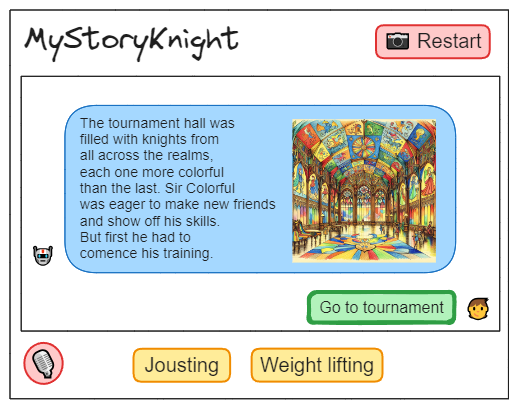
\includegraphics[width=0.45\textwidth]{figures/user-interface.png}
    \caption{Mockup of the user interface.}
    \label{fig:user-interface}
\end{figure}

The system uses a webcam to scan and identify user drawings which are then uploaded and analyzed. The story is then told using speech synthesis with the OpenAI API \cite{20:openai-api}, and story images are generated using DALL-E \cite{21:dalle}. The generated images are optimized to maintain a style similar to that of the user. Actions are then presented to the user, and these could be activated by clicking, or alternatively using voice commands. The user can also choose to restart the story at any point.

\section{Experiencing MyStoryKnight}
\label{subsec:using-mystoryknight}
In this section, we describe the interaction flow of the system.

\vspace{10pt} % Add 10pt of vertical spacing

\begin{quote}
    \textit{Our story begind with a few colord strokes on a piece of paper.}
\end{quote}

\vspace{10pt} % Add 10pt of vertical spacing

The user draws a character on a piece of paper, and the system scans the drawing using a webcam (Fig. \ref{fig:knight}).

\begin{figure}[h]
    \centering
    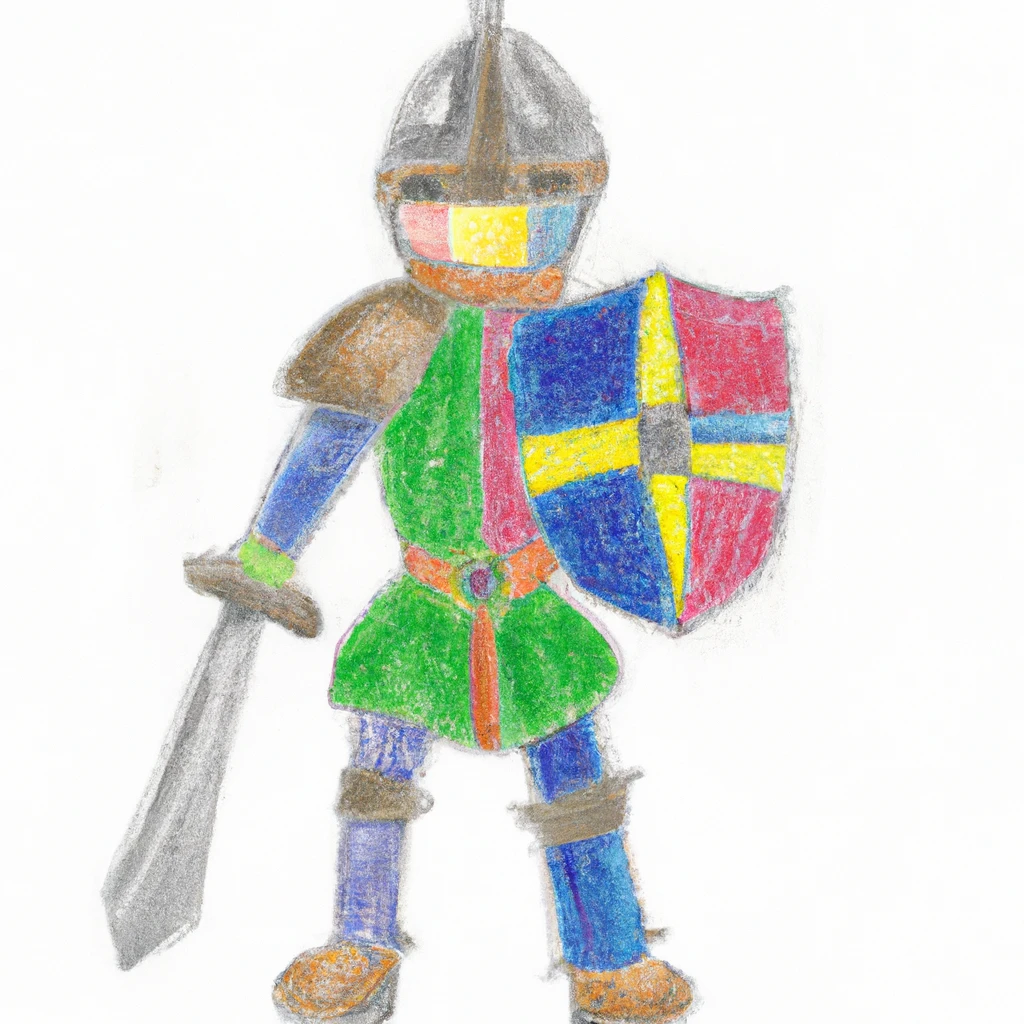
\includegraphics[width=0.3\textwidth]{figures/knight.png}
    \caption{An example of a user drawing. A drawing of a knight, generated with OpenAI's DALL-E \cite{21:dalle}.}
    \label{fig:knight}
\end{figure}

The drawing is then uploaded to the system and analyzed. The system then generates a character description and a background story based on the drawing. The background story is then told to the user.

\vspace{10pt} % Add 10pt of vertical spacing

\begin{quote}
    \textit{Sir Colorful, the most vibrant knight in all the land. Each color on Sir Colorfuls armor and shield represents a virtue: blue for loyalty, yellow for generosity, green for hope, and red for courage. With his trusty sword and shield, Sir Colorful is ready to face any challenge.}
\end{quote}

\vspace{10pt} % Add 10pt of vertical spacing

The user is then presented with a set of actions to choose from: \verb|Go to tournament| or \verb|Run away|. These choices are then fed into GPT-4 to generate the next part of the story, and the next set of actions. The user chooses \verb|Go to tournament| and the story continues (Fig. \ref{fig:tournament}).

\vspace{10pt} % Add 10pt of vertical spacing

\begin{figure}[h]
    \centering
    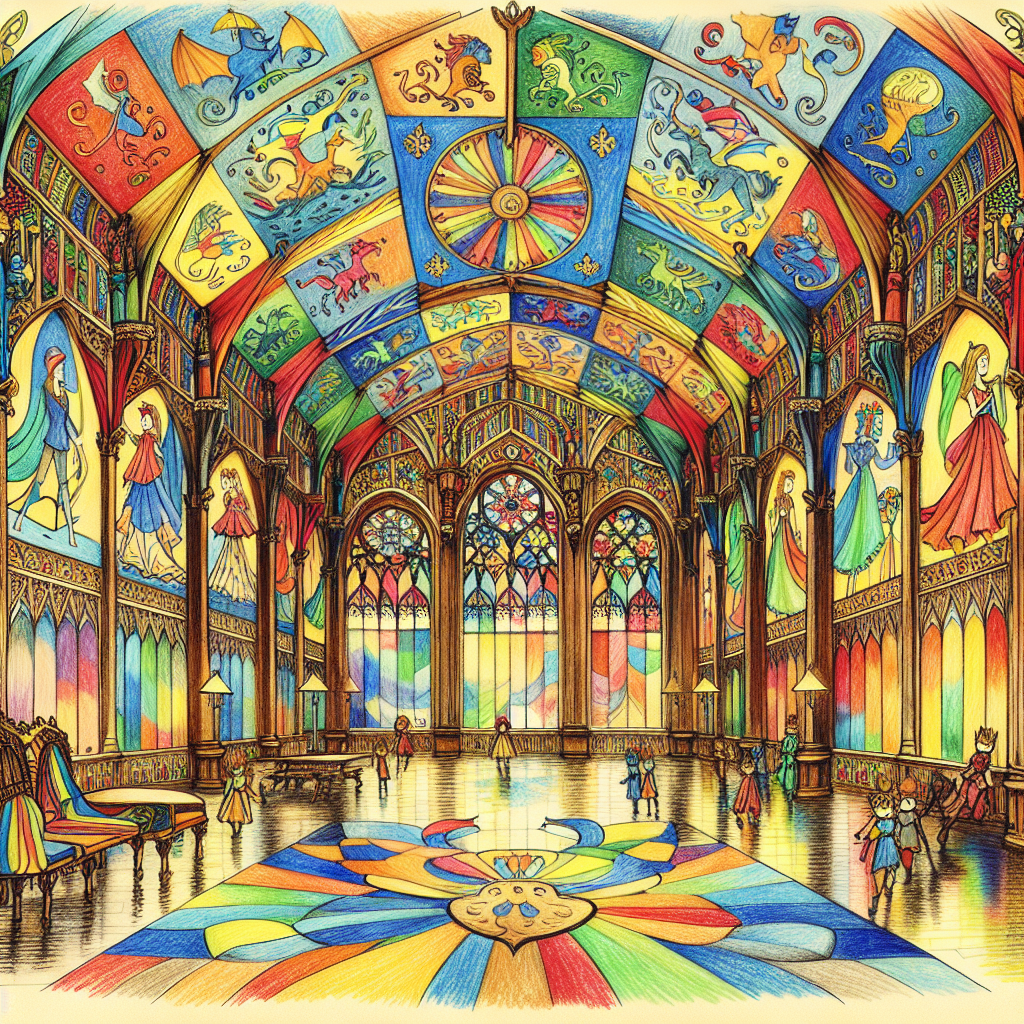
\includegraphics[width=0.35\textwidth]{figures/tournament-hall.png}
    \caption{An example output of the system, the \'tournament hall\'. Generated with OpenAI's DALL-E \cite{21:dalle}.}
    \label{fig:tournament}
\end{figure}

\begin{quote}
    \textit{The tournament hall was filled with knights from all across the realms, each one more colorful than the last. Sir Colorful was eager to make new friends and show off his skills. But first he had to comence his training.}
\end{quote}

\vspace{10pt} % Add 10pt of vertical spacing

This leads to the following actions: \verb|Jousting| and \verb|Weight lifting|. The user makes their choice and the story continues. This process repeats until the user chooses to end the story or the story reaches a maximum number of parts.

%4
\section{Conclusion}
\label{sec:conclusion}
In this paper, we presented \textit{MyStoryKnight}, an interactive storytelling system that uses character drawings as input. We generate an adventure-type story with multiple explorable branches using LLM hallucinations. Additionally, we use a complexity analysis algorithm to guide the LLM hallucinations to generate a coherent and consistent story. We believe that the use of a drawing as input further improves the engagement in the story and characters. In the future we plan to hold a user study to evaluate the effectiveness of our system in promoting creativity and engagement.

% Acknowledgment
% \begin{acknowledgment}
% \end{acknowledgment}

% Bibliography
\bibliographystyle{ipsjsort-e}
\bibliography{references}

% Appendix
% \appendix

\end{document}
